% ============================================================
%  GUÍA 5: ESTRUCTURA ATÓMICA
%  Curso 4to Año — Química
%  Autor: Ing. Gabriel Astudillo
%  Clases cubiertas: 7 a 9
% ============================================================

\documentclass[12pt, a4paper]{article}

% ── Paquetes ─────────────────────────────────────────────────

\usepackage{mathwizards-guia}
\usepackage{float}      % posicionamiento [H]
\usepackage[hidelinks]{hyperref}   % enlaces en atribuciones
\mwguia{Guía 5 — Estructura Atómica}{Ing. Gabriel Astudillo $\cdot$ 4to Año}

\begin{document}
% ============================================================

% ── Portada / Título ─────────────────────────────────────────
\mwportada{Guía de Estudio 5}{Estructura Atómica}{Modelos atómicos, partículas subatómicas, configuración electrónica y números cuánticos}

\vspace{4pt}
\begin{cuadroinfo}
  \small
  \textbf{Presentación:} ¡Hola! ¿Te has preguntado alguna vez de qué está hecha la materia? Todo lo que ves —tu cuaderno, el aire, tú mismo— está formado por \emph{átomos}. Pero ¿cómo es un átomo por dentro? A lo largo de la historia, los científicos han ido construyendo modelos cada vez más precisos: desde la esfera indivisible de Dalton hasta el átomo cuántico actual. En esta guía viajaremos por esa historia, conoceremos las partículas subatómicas, aprenderemos a escribir configuraciones electrónicas y a describir electrones con números cuánticos. ¡Vamos a convertirnos en \emph{exploradores del microcosmos}!
  \\[4pt]
  \textbf{Nivel de Dificultad:}\quad
  \facil{} Básico / Directo \quad
  \medio{} Intermedio \quad
  \dificil{} Desafiante
\end{cuadroinfo}

\vspace{8pt}

% ============================================================
\section{Modelos atómicos, partículas subatómicas y núcleo}
% ============================================================

\subsection{Evolución de los modelos atómicos}

\begin{cuadroteoria}
  \textbf{Línea de tiempo de los modelos atómicos:}
  \begin{center}
    \begin{tabular}{p{2.6cm}p{9.5cm}}
      \toprule
      \textbf{Modelo}        & \textbf{Idea principal}                                                                                                                  \\
      \midrule
      Dalton (1803)          & El átomo es una esfera \emph{indivisible} e \emph{indestructible}.                                                                       \\
      Thomson (1897)         & Descubre el \emph{electrón}; el átomo es una esfera positiva con electrones incrustados (modelo del \emph{pudín de pasas}).              \\
      Rutherford (1911)      & El átomo tiene un \emph{núcleo} pequeño, denso y positivo, y los electrones giran a su alrededor (experimento de la lámina de oro).      \\
      Bohr (1913)            & Los electrones giran en \emph{órbitas} (niveles) con energías fijas.                                                                     \\
      Modelo cuántico actual & Los electrones se describen con \emph{probabilidades}: habitan regiones llamadas \emph{orbitales}; los niveles se dividen en subniveles. \\
      \bottomrule
    \end{tabular}
  \end{center}
\end{cuadroteoria}

\subsection{Partículas subatómicas}

\begin{cuadroteoria}
  \textbf{Las tres partículas fundamentales del átomo:}
  \begin{center}
    \begin{tabular}{lcccc}
      \toprule
      Partícula & Símbolo & Carga & Masa                       & Ubicación            \\
      \midrule
      Protón    & $p^{+}$ & $+1$  & $\approx 1$ u              & Núcleo               \\
      Neutrón   & $n^{0}$ & $0$   & $\approx 1$ u              & Núcleo               \\
      Electrón  & $e^{-}$ & $-1$  & $\approx \frac{1}{1836}$ u & Alrededor del núcleo \\
      \bottomrule
    \end{tabular}
  \end{center}
\end{cuadroteoria}

\begin{cuadroteoria}
  \textbf{Número atómico y número másico:}
  \begin{itemize}[leftmargin=*]
    \item \textbf{Número atómico} ($Z$): cantidad de \textbf{protones} del núcleo. Identifica al elemento.
    \item \textbf{Número másico} ($A$): cantidad de \textbf{protones + neutrones} del núcleo.
  \end{itemize}
  Se escribe en la notación ${}^{A}_{Z}X$ (por ejemplo, ${}^{23}_{11}\text{Na}$):
  \begin{itemize}[leftmargin=*]
    \item Protones $= Z$.
    \item Neutrones $= A - Z$.
    \item Electrones $= Z$ (en el átomo neutro).
  \end{itemize}
\end{cuadroteoria}

\begin{cuadroteoria}
  \textbf{Isótopos e iones:}
  \begin{itemize}[leftmargin=*]
    \item \textbf{Isótopos:} átomos del mismo elemento (mismo $Z$) con distinto $A$ (distinto número de neutrones). Ej.: ${}^{12}_{6}\text{C}$ y ${}^{14}_{6}\text{C}$.
    \item \textbf{Iones:} átomos con carga por ganar o perder electrones:
          \begin{itemize}[leftmargin=*]
            \item \textbf{Catión} (carga $+$): perdió electrones. Ej.: $\text{Na}^{+}$ (11 protones, 10 electrones).
            \item \textbf{Anión} (carga $-$): ganó electrones. Ej.: $\text{Cl}^{-}$ (17 protones, 18 electrones).
          \end{itemize}
  \end{itemize}
\end{cuadroteoria}

\begin{cuadroadvertencia}
  \textbf{Errores clásicos:}
  \begin{itemize}[leftmargin=*]
    \item Confundir $Z$ con $A$: $Z$ son protones (identidad); $A$ es protones + neutrones (masa).
    \item Pensar que los iones ganan o pierden \emph{protones}: no, solo ganan o pierden \emph{electrones}.
    \item Calcular neutrones como $Z - A$: la fórmula correcta es $A - Z$ (y el resultado siempre es positivo).
  \end{itemize}
\end{cuadroadvertencia}

\subsection{Ejercicios resueltos}

\textbf{Ejemplo R1.} El sodio tiene $Z = 11$ y $A = 23$. ¿Cuántos protones, neutrones y electrones tiene un átomo neutro de sodio?

\begin{cuadrosolucion}
  \textbf{Solución:}
  \begin{itemize}
    \item Protones $= Z = 11$.
    \item Neutrones $= A - Z = 23 - 11 = 12$.
    \item Electrones $= Z = 11$ (átomo neutro).
  \end{itemize}
\end{cuadrosolucion}

\textbf{Ejemplo R2.} Escribe la notación ${}^{A}_{Z}X$ del átomo con 26 protones y 30 neutrones, e indica cuántos electrones tiene en estado neutro.

\begin{cuadrosolucion}
  \textbf{Solución:} $Z = 26$ y $A = 26 + 30 = 56$; el elemento es el hierro (Fe):
  $${}^{56}_{26}\text{Fe} \qquad \text{con 26 electrones en estado neutro.}$$
\end{cuadrosolucion}

\textbf{Ejemplo R3.} Compara los isótopos ${}^{12}_{6}\text{C}$ y ${}^{14}_{6}\text{C}$. ¿Qué tienen igual y qué diferente?

\begin{cuadrosolucion}
  \textbf{Solución:} ambos tienen $Z = 6$: 6 protones y 6 electrones. Difieren en los neutrones: el ${}^{12}\text{C}$ tiene $12 - 6 = 6$ neutrones y el ${}^{14}\text{C}$ tiene $14 - 6 = 8$ neutrones.
\end{cuadrosolucion}

\textbf{Ejemplo R4.} El ion $\text{Ca}^{2+}$ tiene $Z = 20$. ¿Cuántos protones y electrones tiene?

\begin{cuadrosolucion}
  \textbf{Solución:} los protones no cambian: $20$ protones. La carga $2+$ indica que perdió 2 electrones: $20 - 2 = 18$ electrones.
\end{cuadrosolucion}

\subsection{Ejercicios propuestos}

\begin{enumerate}[leftmargin=*, resume]
  \item \facil{} ¿Quién propuso que el átomo tiene un núcleo pequeño y positivo? ¿Con qué experimento?

  \item \facil{} Escribe las tres partículas subatómicas con su carga.

  \item \facil{} ¿Qué número identifica al elemento: $Z$ o $A$? ¿Qué indica cada uno?

  \item \facil{} Un átomo tiene $Z = 8$ y $A = 16$. ¿Cuántos protones, neutrones y electrones tiene?

  \item \facil{} Escribe la notación ${}^{A}_{Z}X$ de un átomo con 19 protones y 20 neutrones.

  \item \medio{} El aluminio tiene $Z = 13$ y $A = 27$. Calcula protones, neutrones y electrones.

  \item \medio{} ¿En qué se diferencian los isótopos ${}^{35}_{17}\text{Cl}$ y ${}^{37}_{17}\text{Cl}$? Calcula sus neutrones.

  \item \medio{} El ion $\text{O}^{2-}$ tiene $Z = 8$. ¿Cuántos protones y electrones tiene?

  \item \medio{} El ion $\text{Mg}^{2+}$ tiene $Z = 12$. ¿Cuántos electrones tiene? ¿Es un catión o un anión?

  \item \dificil{} Un átomo neutro tiene 26 electrones y 30 neutrones. ¿Cuál es su $Z$, su $A$ y su notación?

  \item \dificil{} Un ion con carga $3+$ tiene 13 protones. ¿Cuántos electrones tiene? ¿Qué elemento es si $Z = 13$?
\end{enumerate}

% ============================================================
\section{Configuración electrónica}
% ============================================================

\subsection{Niveles, subniveles y orbitales}

\begin{cuadroteoria}
  Los electrones se organizan en \textbf{niveles} de energía (numerados $1, 2, 3, \ldots$). Cada nivel se divide en \textbf{subniveles} ($s$, $p$, $d$, $f$), y cada subnivel en \textbf{orbitales} (regiones donde es probable encontrar al electrón).
  \begin{center}
    \begin{tabular}{lcccc}
      \toprule
      Subnivel & Orbitales & Capacidad (electrones) & Nivel & Capacidad total \\
      \midrule
      $s$      & 1         & 2                      & 1     & 2               \\
      $p$      & 3         & 6                      & 2     & 8               \\
      $d$      & 5         & 10                     & 3     & 18              \\
      $f$      & 7         & 14                     & 4     & 32              \\
      \bottomrule
    \end{tabular}
  \end{center}
\end{cuadroteoria}

\begin{cuadroteorianobg}
  \textbf{Forma de los orbitales:} cada tipo de subnivel tiene una geometría característica que representa la región del espacio donde es probable encontrar al electrón.

  \begin{figure}[H]
    \centering
    \begin{minipage}[t]{0.22\textwidth}
      \centering
      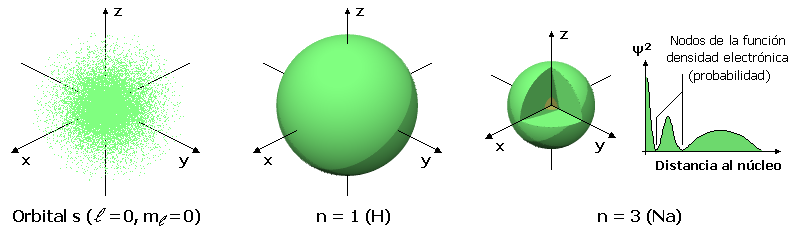
\includegraphics[width=\linewidth]{orbital_s.png}\\[2pt]
      \textbf{Orbital $s$}\\
      {\tiny Esférico. 1 orbital, 2 e$^-$.\\
      \textit{Orbital Viewer}, D.~Manthey (GFDL).}
    \end{minipage}\hfill
    \begin{minipage}[t]{0.22\textwidth}
      \centering
      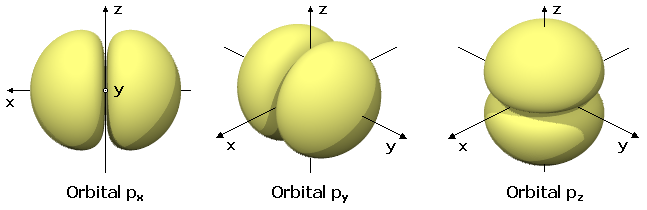
\includegraphics[width=\linewidth]{orbital_p.png}\\[2pt]
      \textbf{Orbital $p$}\\
      {\tiny Bilobular. 3 orbitales, 6 e$^-$.\\
      \textit{Orbital Viewer}, D.~Manthey (GFDL).}
    \end{minipage}\hfill
    \begin{minipage}[t]{0.27\textwidth}
      \centering
      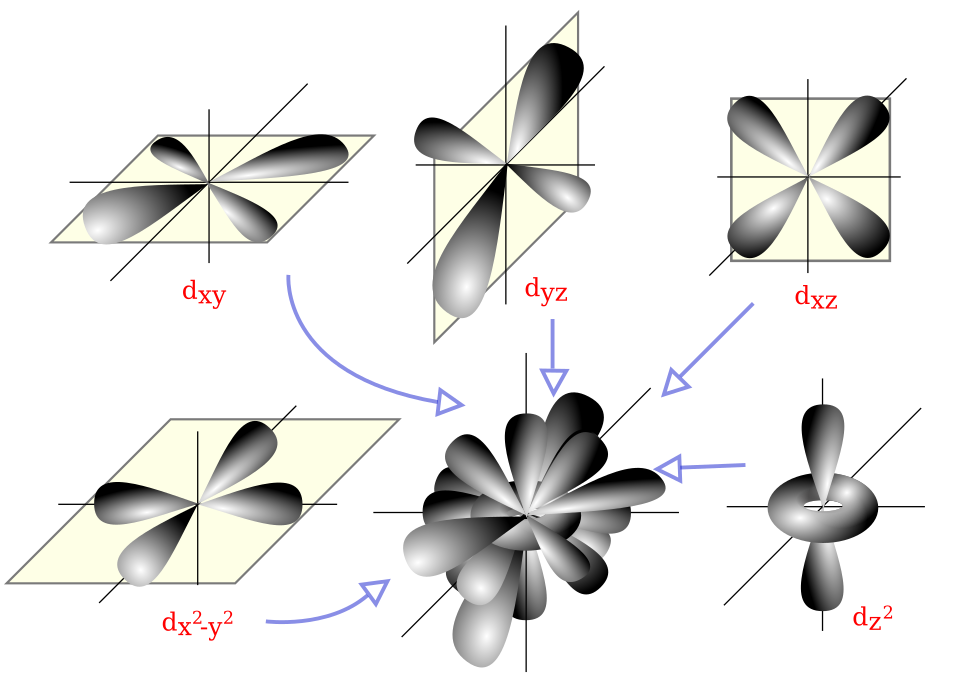
\includegraphics[width=\linewidth]{orbital_d.png}\\[2pt]
      \textbf{Orbitales $d$}\\
      {\tiny 5 orbitales, 10 e$^-$.\\
      \href{https://commons.wikimedia.org/wiki/File:D_orbitals.svg}{Wikimedia Commons} (CC~BY-SA).}
    \end{minipage}\hfill
    \begin{minipage}[t]{0.22\textwidth}
      \centering
      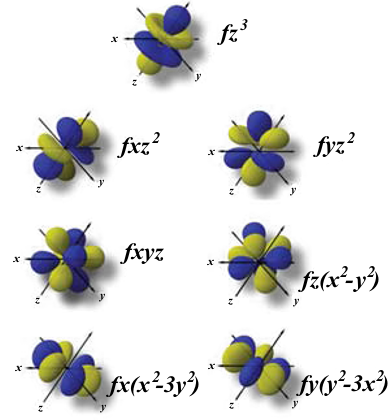
\includegraphics[width=\linewidth]{orbital_f.png}\\[2pt]
      \textbf{Orbitales $f$}\\
      {\tiny 7 orbitales, 14 e$^-$.\\
      Terrón, García-Raso \& Barceló-Oliver\\(CC~BY-SA~3.0, Wikimedia Commons).}
    \end{minipage}
  \end{figure}
\end{cuadroteorianobg}

\newpage

\begin{cuadroteoria}
  \textbf{Principios que gobiernan la configuración electrónica:}
  \begin{itemize}[leftmargin=*]
    \item \textbf{Principio de Aufbau} (diagrama de Moeller): los electrones llenan primero los subniveles de menor energía.
    \item \textbf{Principio de exclusión de Pauli:} en un mismo átomo no pueden existir dos electrones con los cuatro números cuánticos iguales (un orbital aloja como máximo 2 electrones con espines opuestos).
    \item \textbf{Regla de Hund:} al llenar un subnivel, primero se colocan electrones sueltos (espines paralelos) y luego se aparean.
  \end{itemize}
\end{cuadroteoria}

\begin{cuadroteorianobg}
  \textbf{Diagrama de Moeller (regla de las diagonales):}
  \begin{center}
    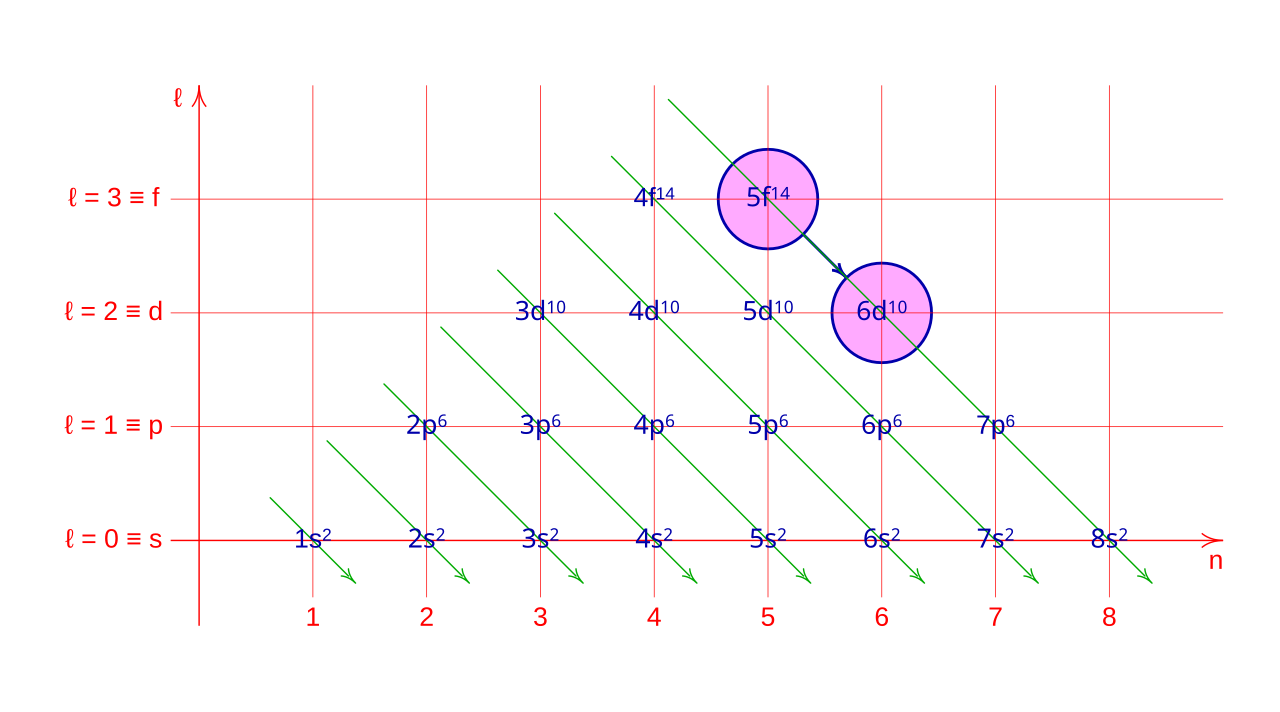
\includegraphics[width=0.52\linewidth]{diagrama_moeller.png}
  \end{center}
  \emph{Truco:} sigue las flechas diagonales de arriba hacia abajo para obtener el orden correcto de llenado ($1s \to 2s \to 2p \to 3s \to 3p \to 4s \to 3d \to \dots$).
\end{cuadroteorianobg}

\begin{cuadropasos}
  \textbf{Escribir una configuración electrónica:}
  \begin{enumerate}[leftmargin=*]
    \item Cuenta los electrones: $Z$ (o $Z \pm$ carga para iones).
    \item Sigue el orden de Moeller llenando cada subnivel hasta su capacidad.
    \item Detente cuando hayas colocado todos los electrones.
    \item Los \textbf{electrones de valencia} son los del último nivel ($n$ mayor): determinan la reactividad y el grupo.
  \end{enumerate}
\end{cuadropasos}

\begin{cuadroadvertencia}
  \textbf{Errores clásicos:}
  \begin{itemize}[leftmargin=*]
    \item Llenar $3d$ antes que $4s$: el orden es $4s$ primero (menor energía).
    \item Superar la capacidad de un subnivel: $p$ máximo 6 electrones, $d$ máximo 10.
    \item Confundir electrones de valencia con el número total de electrones: la valencia es solo el último nivel.
  \end{itemize}
\end{cuadroadvertencia}

\newpage

\subsection{Ejercicios resueltos}

\textbf{Ejemplo R1.} Escribe la configuración electrónica del oxígeno ($Z = 8$).

\begin{cuadrosolucion}
  \textbf{Solución:} llenamos siguiendo el diagrama de Moeller:
  $$1s^{2} \; 2s^{2} \; 2p^{4}$$
  Total: $2 + 2 + 4 = 8$ electrones. \checkmark \ Los electrones de valencia son los del nivel 2: $2 + 4 = 6$.
\end{cuadrosolucion}

\textbf{Ejemplo R2.} Escribe la configuración electrónica del potasio ($Z = 19$).

\begin{cuadrosolucion}
  \textbf{Solución:}
  $$1s^{2} \; 2s^{2} \; 2p^{6} \; 3s^{2} \; 3p^{6} \; 4s^{1}$$
  Total: $2 + 2 + 6 + 2 + 6 + 1 = 19$. \checkmark \ El potasio tiene 1 electrón de valencia (en el nivel 4).
\end{cuadrosolucion}

\textbf{Ejemplo R3.} ¿Cuántos electrones de valencia tiene el cloro ($Z = 17$)?

\begin{cuadrosolucion}
  \textbf{Solución:} su configuración es $1s^{2} 2s^{2} 2p^{6} 3s^{2} 3p^{5}$. El último nivel es el 3: $3s^{2}3p^{5}$ aporta $2 + 5 = 7$ electrones de valencia.
\end{cuadrosolucion}

\subsection{Ejercicios propuestos}

\begin{enumerate}[leftmargin=*, resume]
  \item \facil{} ¿Cuántos electrones caben en un orbital? ¿Cuántos orbitales tiene el subnivel $p$?

  \item \facil{} Escribe la configuración electrónica del helio ($Z = 2$).

  \item \facil{} Escribe la configuración electrónica del neón ($Z = 10$).

  \item \facil{} ¿Qué subnivel se llena antes: $3d$ o $4s$? ¿Por qué?

  \item \medio{} Escribe la configuración electrónica del sodio ($Z = 11$) e indica sus electrones de valencia.

  \item \medio{} Escribe la configuración electrónica del calcio ($Z = 20$).

  \item \medio{} ¿Cuántos electrones de valencia tiene el azufre ($Z = 16$)?

  \item \medio{} ¿Cuántos electrones hay en el nivel 3 del argón ($Z = 18$)? (Configúralo primero.)

  \item \dificil{} Escribe la configuración del fósforo ($Z = 15$) y dibuja (con cajas y flechas) los orbitales $3p$ según la regla de Hund.

  \item \dificil{} Un átomo tiene configuración $1s^{2}2s^{2}2p^{6}3s^{2}3p^{4}$. ¿Qué elemento es? (Suma los electrones y compara con $Z$.)

  \item \dificil{} \textbf{El reto de los campeones:} el ion $\text{S}^{2-}$ proviene del azufre ($Z = 16$). Escribe su configuración electrónica (recuerda: ganó 2 electrones) y compárala con la del argón ($Z = 18$). ¿Qué observas?
\end{enumerate}

\newpage

% ============================================================
\section{Números cuánticos y tabla periódica}
% ============================================================

\subsection{Los cuatro números cuánticos}

\begin{cuadroteoria}
  Cada electrón de un átomo se describe con \textbf{cuatro números cuánticos}:
  \begin{center}
    \begin{tabular}{lll}
      \toprule
      Número cuántico & Qué indica        & Valores posibles                           \\
      \midrule
      Principal $n$   & Nivel de energía  & $1, 2, 3, 4, \ldots$                       \\
      Azimutal $l$    & Subnivel          & $0$ ($s$), $1$ ($p$), $2$ ($d$), $3$ ($f$) \\
      Magnético $m_l$ & Orbital           & de $-l$ a $+l$                             \\
      Espín $m_s$     & Giro del electrón & $+\tfrac{1}{2}$ o $-\tfrac{1}{2}$          \\
      \bottomrule
    \end{tabular}
  \end{center}
  Por ejemplo, para el subnivel $2p$: $n = 2$, $l = 1$ y $m_l$ puede ser $-1$, $0$ o $+1$ (tres orbitales).
\end{cuadroteoria}

\begin{cuadropasos}
  \textbf{Determinar los números cuánticos del último electrón:}
  \begin{enumerate}[leftmargin=*]
    \item Escribe la configuración electrónica.
    \item Identifica el último subnivel ocupado y cuántos electrones tiene ($n$ y $l$).
    \item Asigna $m_l$ recorriendo los orbitales de izquierda a derecha ($-l, \ldots, 0, \ldots, +l$) y $m_s$ siguiendo la regla de Hund (primero $+\tfrac{1}{2}$, luego $-\tfrac{1}{2}$).
  \end{enumerate}
\end{cuadropasos}

\subsection{Relación con la tabla periódica}

\begin{cuadroteoria}
  \begin{itemize}[leftmargin=*]
    \item El \textbf{periodo} (fila) coincide con el número del último nivel ($n$) ocupado.
    \item El \textbf{grupo} (columna) se relaciona con los electrones de valencia:
          \begin{itemize}[leftmargin=*]
            \item Grupos 1 y 2: 1 y 2 electrones de valencia.
            \item Grupos 13 a 18: valencia $= $ número del grupo $- 10$.
          \end{itemize}
    \item Los elementos del mismo grupo comparten el número de electrones de valencia y, por tanto, propiedades químicas parecidas.
  \end{itemize}
\end{cuadroteoria}

\begin{cuadroadvertencia}
  \textbf{Errores clásicos:}
  \begin{itemize}[leftmargin=*]
    \item Asignar $l = n$: el azimutal depende del \emph{subnivel}, no del nivel ($n = 3$ puede tener $l = 0, 1, 2$).
    \item Confundir $m_l$ con $m_s$: $m_l$ ubica el orbital; $m_s$ describe el espín.
    \item Olvidar que en un subnivel medio lleno los primeros electrones van sueltos (Hund) antes de aparearse.
  \end{itemize}
\end{cuadroadvertencia}

\subsection{Ejercicios resueltos}

\textbf{Ejemplo R1.} Determina los números cuánticos del último electrón del nitrógeno ($Z = 7$).

\begin{cuadrosolucion}
  \textbf{Solución:} configuración: $1s^{2}2s^{2}2p^{3}$.
  \begin{itemize}
    \item Último subnivel: $2p$ $\Rightarrow$ $n = 2$, $l = 1$.
    \item Los tres electrones $2p$ se colocan sueltos (Hund): orbitales $-1$, $0$, $+1$, todos con espín $+\tfrac{1}{2}$.
    \item El último electrón ocupa el orbital $m_l = +1$ con $m_s = +\tfrac{1}{2}$.
  \end{itemize}
  Números cuánticos: $(n, l, m_l, m_s) = (2, 1, +1, +\tfrac{1}{2})$.
\end{cuadrosolucion}

\textbf{Ejemplo R2.} ¿En qué periodo y grupo de la tabla periódica está el cloro ($Z = 17$)?

\begin{cuadrosolucion}
  \textbf{Solución:} configuración: $1s^{2}2s^{2}2p^{6}3s^{2}3p^{5}$.
  \begin{itemize}
    \item Último nivel: $3$ $\Rightarrow$ periodo 3.
    \item Electrones de valencia: $2 + 5 = 7$ $\Rightarrow$ grupo 17 (7A).
  \end{itemize}
  El cloro está en el periodo 3, grupo 17.
\end{cuadrosolucion}

\textbf{Ejemplo R3.} El magnesio tiene configuración $1s^{2}2s^{2}2p^{6}3s^{2}$. ¿Cuántos electrones de valencia tiene y en qué grupo está?

\begin{cuadrosolucion}
  \textbf{Solución:} el último nivel es el 3 y solo tiene el subnivel $3s$ con 2 electrones: 2 electrones de valencia. Está en el grupo 2 (metales alcalinotérreos).
\end{cuadrosolucion}

\newpage %ajuste para pág

\subsection{Ejercicios propuestos}

\begin{enumerate}[leftmargin=*, resume]
  \item \facil{} ¿Qué indica el número cuántico principal $n$? ¿Y el azimutal $l$?

  \item \facil{} ¿Qué valores puede tomar $m_l$ si $l = 0$? ¿Y si $l = 1$?

  \item \facil{} ¿Cuántos orbitales tiene el subnivel $2p$? ¿Cuántos electrones aloja como máximo?

  \item \medio{} Determina los números cuánticos del último electrón del boro ($Z = 5$).

  \item \medio{} Determina los números cuánticos del último electrón del oxígeno ($Z = 8$).

  \item \medio{} ¿En qué periodo y grupo está el sodio ($Z = 11$)? (Configúralo primero.)

  \item \medio{} ¿Cuántos electrones de valencia tiene el aluminio ($Z = 13$) y en qué grupo está?

  \item \dificil{} Determina los números cuánticos del último electrón del fósforo ($Z = 15$) aplicando la regla de Hund.

  \item \dificil{} Un elemento está en el periodo 3, grupo 16. ¿Cuál es su configuración electrónica y su $Z$?

  \item \dificil{} El último electrón de un elemento tiene números cuánticos $(3, 1, -1, +\tfrac{1}{2})$. Escribe su configuración e identifica el elemento.

  \item \dificil{} \textbf{El reto de los campeones:} el hierro ($Z = 26$) tiene configuración $1s^{2}2s^{2}2p^{6}3s^{2}3p^{6}4s^{2}3d^{6}$. a) ¿Cuántos electrones de valencia tiene? b) Determina los números cuánticos del último electrón del subnivel $3d$. (Pista: recuerda la regla de Hund para los orbitales $d$: $-2, -1, 0, +1, +2$.)
\end{enumerate}

\newpage

% ============================================================
\section{Clave de Respuestas}
% ============================================================

\subsection*{Sección 1: Modelos atómicos y partículas subatómicas (Ejercicios 1--11)}

\begin{enumerate}[leftmargin=*, label=\textbf{\arabic*.}]
  \setcounter{enumi}{0}
  \item Rutherford, con el experimento de la lámina de oro.
  \item Protón ($+1$), neutrón ($0$) y electrón ($-1$).
  \item $Z$ identifica al elemento (protones); $A$ es protones + neutrones.
  \item 8 protones, 8 neutrones ($16 - 8$) y 8 electrones.
  \item ${}^{39}_{19}\text{K}$.
  \item 13 protones, $27 - 13 = 14$ neutrones y 13 electrones.
  \item Ambos tienen 17 protones; el ${}^{35}\text{Cl}$ tiene 18 neutrones y el ${}^{37}\text{Cl}$ tiene 20.
  \item 8 protones y $8 + 2 = 10$ electrones (ganó 2).
  \item $12 - 2 = 10$ electrones; es un catión.
  \item $Z = 26$, $A = 26 + 30 = 56$: ${}^{56}_{26}\text{Fe}$.
  \item $13 - 3 = 10$ electrones; es el aluminio (Al).
\end{enumerate}

\subsection*{Sección 2: Configuración electrónica (Ejercicios 12--22)}

\begin{enumerate}[leftmargin=*, label=\textbf{\arabic*.}]
  \setcounter{enumi}{11}
  \item 2 electrones por orbital; el subnivel $p$ tiene 3 orbitales.
  \item $1s^{2}$.
  \item $1s^{2}2s^{2}2p^{6}$.
  \item $4s$: tiene menor energía según el diagrama de Moeller.
  \item $1s^{2}2s^{2}2p^{6}3s^{1}$; 1 electrón de valencia.
  \item $1s^{2}2s^{2}2p^{6}3s^{2}3p^{6}4s^{2}$.
  \item $1s^{2}2s^{2}2p^{6}3s^{2}3p^{4}$: 6 electrones de valencia.
  \item Nivel 3: $3s^{2}3p^{6}$: 8 electrones.
  \item $1s^{2}2s^{2}2p^{6}3s^{2}3p^{3}$; en $3p$ los tres electrones van sueltos ($\uparrow\,\uparrow\,\uparrow$).
  \item Suma $2+2+6+2+4 = 16$: es el azufre (S).
  \item \textbf{Reto:} $\text{S}^{2-}$ tiene 18 electrones: $1s^{2}2s^{2}2p^{6}3s^{2}3p^{6}$, igual que el argón (configuración isoelectrónica).
\end{enumerate}

\subsection*{Sección 3: Números cuánticos y tabla periódica (Ejercicios 23--33)}

\begin{enumerate}[leftmargin=*, label=\textbf{\arabic*.}]
  \setcounter{enumi}{22}
  \item $n$ indica el nivel de energía; $l$ indica el subnivel ($0=s$, $1=p$, $2=d$, $3=f$).
  \item Si $l = 0$: solo $m_l = 0$. Si $l = 1$: $m_l = -1, 0, +1$.
  \item 3 orbitales; máximo 6 electrones.
  \item Boro: $1s^{2}2s^{2}2p^{1}$: $(n,l,m_l,m_s) = (2, 1, -1, +\tfrac{1}{2})$.
  \item Oxígeno: $2p^{4}$: orbitales $-1, 0$ llenos y $+1$ con un par: último electrón $(2, 1, +1, -\tfrac{1}{2})$.
  \item Sodio: $3s^{1}$: periodo 3, grupo 1.
  \item $3s^{2}3p^{1}$: 3 electrones de valencia; grupo 13.
  \item Fósforo: $3p^{3}$ sueltos en $-1, 0, +1$: último electrón $(3, 1, +1, +\tfrac{1}{2})$.
  \item Periodo 3, grupo 16: $1s^{2}2s^{2}2p^{6}3s^{2}3p^{4}$; $Z = 16$ (azufre).
  \item $(3, 1, -1, +\tfrac{1}{2})$: último en $3p$: $1s^{2}2s^{2}2p^{6}3s^{2}3p^{1}$; $Z = 13$ (aluminio).
  \item \textbf{Reto:} a) 2 electrones de valencia ($4s^{2}$). b) Subnivel $3d$ con 6 electrones: se llenan $-2, -1, 0, +1, +2$ sueltos (5) y el sexto se aparea en $-2$: último electrón $(3, 2, -2, -\tfrac{1}{2})$.
\end{enumerate}

\vspace{8pt}
\begin{cuadroinfo}
  \small
  \textbf{¿Cómo te fue?} Ya conoces el interior del átomo: sus partículas, cómo se acomodan los electrones y cómo describirlos. Con estas bases, en la próxima guía aprenderemos a \emph{contar} la materia: el mol, el balanceo de ecuaciones y la estequiometría. ¡Nos vemos ahí!
\end{cuadroinfo}

\end{document}
